Algoritma Floyd-Warshall adalah salah satu varian dari pemrograman dinamis, yaitu suatu metode yang melakukan pemecahan dengan memandang solusi yang akan diperoleh sebagai suatu keputusan yang saling terkait. Artinya solusi-solusi tersebut dibentuk dari solusi yang berasal dari tahap sebelumnya dan ada kemungkinan solusi lebih dari satu Algoritma Floyd Warshall adalah dengan membandingkan semua lintasan yang mungkin terjadi dalam graf untuk setiap pasang simpul dan melakukan pengujian dari setiap kombinasi simpul yang diperoleh \cite{novianti2019implementasi}.

\section{Algoritma Floyd Warshall}
Algoritma Floyd-Warshall adalah salah satu varian dari pemrograman dinamis, yaitu suatu metode yang melakukan pemecahan dengan memandang solusi yang akan diperoleh sebagai suatu keputusan yang saling terkait. Artinya solusi-solusi tersebut dibentuk dari solusi yang berasal dari tahap sebelumnya dan ada kemungkinan solusi lebih dari satu Algoritma Floyd Warshall adalah dengan membandingkan semua lintasan yang mungkin terjadi dalam graf untuk setiap pasang simpul dan melakukan pengujian dari setiap kombinasi simpul yang diperoleh \cite{novianti2019implementasi}.
Algoritma Floyd Warshall ditemukan oleh Warshall untuk mencari path terpendek merupakan algoritma yang sederhana dan mudah implementasikannya. Algoritma Floyd Warshall adalah matriks hubung graf berarah berlabel, dan keluarannya adalah path terpendek dari semua titik kesemua titik. Dalam usaha mencari jalur terpendek, algoritma Warshall memulai iterasi dari titik awalnya kemudian memperpanjang path dengan mengevaluasi titik demi titik hingga mencapai titik tujuan dengan jumlah bobot yang seminimum mungkin \cite{hasibuan2016penerapan}.
mekanisme dari algoritma FloydWarshall ini terdiri dari beberapa langkah yang harus dilakukan, yaitu \cite{darnita2017implementasi}:
\begin{enumerate}
    \item Langkah awal yang harus dilakukan untuk menentukan shortest path dengan menggunakan algoritma Floyd-Warshall adalah dengan merepresentasikan suatu graf sebagai suatu matriks berbobot.
    \item Langkah kedua adalah melakukan dekomposisi.
    \item Langkah ketiga adalah menentukan struktur shortest path. Dalam hal ini, harus dilakukan dua pengamatan terlebih dahulu sebelum melangkah lebih jauh.
    \item Dilakukan penentuan shortest path
    \item Melakukan iterasi yang dimulai dari iterasi ke 0 sampai dengan.
\end{enumerate}

Hasil akhir dari algoritma Floyd-Warshall adalah matriks untuk iterasi ke-n. Dari matriks ken ini, dapat dilihat shortest path untuk setiap vertex pada suatu graph.

Misalkan terdapat suatu graf G dengan simpul-simpul V yang  masing-masing  bernomor  1  s.d.  N  (sebanyak  N  buah).      Misalkan      pula      terdapat      suatu      fungsi      shortestPath(i,   j,   k)    yang    mengembalikan    kemungkinan  jalur  terpendek  dari  i  ke  j  dengan  hanya  memanfaatkan simpul 1 s.d. k sebagai titik perantara. Tujuan   akhir   penggunaan   fungsi   ini   adalah   untuk   mencari  jalur  terpendek  dari  setiap  simpul  i  ke  simpul  j  dengan perantara simpul 1 s.d. k+1. 

Ada dua kemungkinan yang terjadi:  
\begin{enumerate}
    \item Jalur terpendek yang sebenarnya hanya berasal dari simpul-simpul yang berada antara 1 hingga k. 
    \item Ada sebagian jalur yang berasal dari simpul-simpul i s.d. k+1, dan juga dari k+1 hingga j.
\end{enumerate}{}

Perlu  diketahui  bahwa  jalur  terpendek  dari  i  ke  j  yang  hanya  melewati  simpul  1  s.d.  k  telah  didefinisikan  pada  fungsi  shortestPath(i,  j,  k)  dan  telah  jelas  bahwa  jika  ada  solusi  dari  i  s.d.  k+1  hingga  j,  maka  panjang  dari  solusi  tadi adalah jumlah (konkatenasi) dari jalur terpendek dari i s.d. k+1 (yang melewati simpul-simpul 1 s.d. k), dan jalur terpendek  dari  k+1  s.d.  j  (juga  menggunakan  simpul-simpul dari 1 s.d. k).

Maka  dari  itu,  rumus  untuk  fungsi  shortestPath(i, j, k) bisa ditulis sebagai:
\begin{equation}
    \label{label21}
    X[i,j] ≤ X[i,k] + X[k,j]
\end{equation}
    \par Keterangan \ref{label21}:
        \par X = Matriks
        \par i = titik awal
        \par j = titik akhir
        \par k = iterasi 1 sampai ke n

Algoritma ini bertujuan untuk menemukan jalur
terpendek berdasarkan bobot terkecil dari satu titik ke titik
lainnya. Misalkan titik mengambarkan gedung dan garis
menggambarkan jalan, maka algoritma Dijkstra melakukan
kalkulasi terhadap semua kemungkinan bobot terkecil dari
setiap titik.

\section{Perhitungan Algoritma Floyd Warshall}
\subsection{Analisis Algoritma Floyd Warshall}
Algoritma Floyd Warshall sangat efisien dari sudut pandang penyimpanan data kare-na dapat diimplementasikan dengan hanya pengubahan sebuah matriks jarak. Adapun mekanisme dari algoritma Floyd-Warshall ini terdiri dari beberapa langkah yang harus dilakukan, yaitu:

\begin{enumerate}
    \item Langkah awal yang harus dilakukan untuk menentukan shortest path dengan menggunakan algoritma Floyd Warshall adalah dengan merepresentasikan suatu graf sebagai suatu matriks berbobot (dapat dilihat pada bagian \ref{pemodelan_graf}).
    \item Langkah kedua adalah melakukan dekomposisi Floyd-Warshall atau membentuk sebuah table matriks dan titik yang akan dihitung (dapat dilihat pada bagian \ref{pemodelan_graf}).
    
    \begin{enumerate}
        \item Hasil yang didapatkan dari graf adalah
            \begin{verbatim}
                K	=	0, 1, 2, 3, 4, 5, 6, 7
                i	=	0, 1, 2, 3, 4, 5, 6, 7
                j	=	0, 1, 2, 3, 4, 5, 6, 7
            \end{verbatim}
        
        \item Untuk rumus yang digunakan:
            \begin{equation}
                Rumus X[i,j] < X[i,k] + X[k,j]
            \end{equation}
            \par Penjelasan lebih dapat dilihat pada point \ref{label21}.
        
        \item Untuk table matriks hubungan graf, terdapat tujuh table Matriks hubungan graf, dimana setiap table meilihki proses yang sama namun dengan nilai matriks yang berubah-ubah. Adapun table matriks yang dihasilkan diberi penamaan dengan table matriks hubungan graf.
        
        \item Langkah selanjutnya, menentukan struktur shortest path kemudian melaku-kan penentuan shortest path dari i ke j yang memuat vertex k.


    \begin{enumerate}
    \item Matriks hubungan graf, K=0:            \begin{table}[!htbp]
    \centering
    \caption{Matriks hubungan graf, K=0}
    \label{table52}
    \begin{tabular}{|l|l|l|l|l|l|l|l|l|}                \hline
         X0 & V0 & V1 & V2 & V3 & V4 & V5 & V6 & V7 \\
    \hline
         V0 & 0 & 543 & - & - & - & 742 & - & - \\
    \hline
          V1 & - & 0 & 1827 & - & 945 & - & - & - \\
    \hline
         V2 & - & - & 0 & 1119 & - & - & - & - \\
    \hline
         V3 & - & - & - & 0 & - & - & - & 647 \\
    \hline
         V4 & - & - & - & 1152 & 0 & - & - & - \\
    \hline
        V5 & - & - & - & - & - & 0 & 778 & - \\
    \hline
        V6 & - & - & - & - & - & 0 & 28.93 & - \\
    \hline
        V7 & - & - & - & - & - & 0 & - & - \\
    \hline
    \end{tabular}
    \end{table}


            \par Penyelesaian:
            \begin{figure}[h]
            \centering
            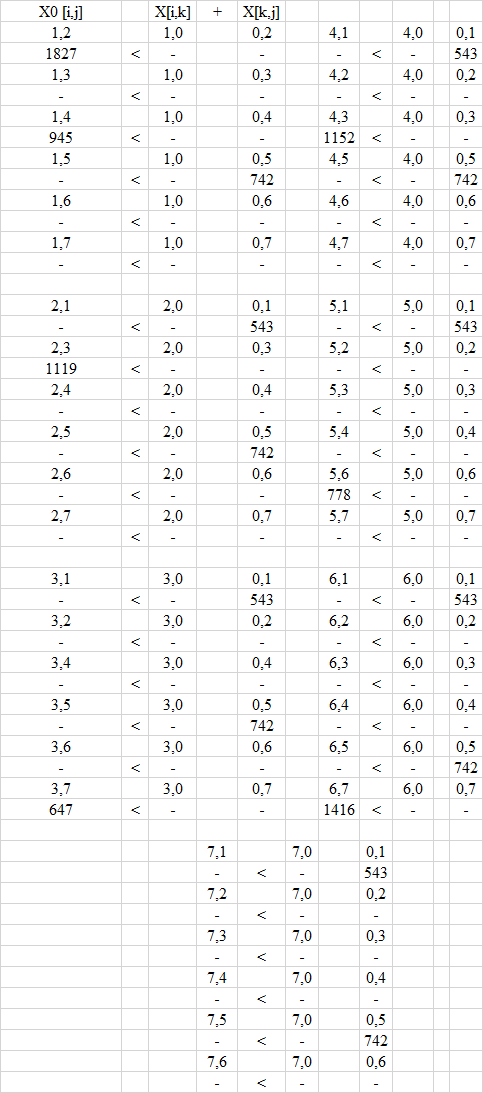
\includegraphics[scale=0.34]{figures/ALGORITMA/MATRIKSX0.png}
            \caption{Matriks X0}
            \label{gambar31}
            \end{figure}
            \par Untuk iterasi terhadap matriks K=0 tidak terdapat jalur dan setiap sel matriks W dicek apakah \verb|X[i,j] < X[i,k] + X[k,j]| jika ya maka \verb|X[i,j]| digannti dengan \verb|X[i,k] + X[k,j]|


            \item Matriks hubungan graf, K=1:
                \begin{table}[!htbp]
                \centering
                \caption{Matriks hubungan graf, K=1}
                \label{table32}
                    \begin{tabular}{|l|l|l|l|l|l|l|l|l|}
                    \hline
                        X1 & V0 & V1 & V2 & V3 & V4 & V5 & V6 & V7 \\
                    \hline
                        V0 & 0 & 543 & 2370 & - & 1488 & 742 & - & - \\
                    \hline
                        V1 & - & 0 & 1827 & - & 945 & - & - & - \\
                    \hline
                        V2 & - & - & 0 & 1119 & - & - & - & - \\
                    \hline
                        V3 & - & - & - & 0 & - & - & - & 647 \\
                    \hline
                        V4 & - & - & - & 1152 & 0 & - & - & - \\
                    \hline
                        V5 & - & - & - & - & - & 0 & 778 & - \\
                    \hline
                       V6 & - & - & - & - & - & 0 & 28.93 & - \\
                    \hline
                       V7 & - & - & - & - & - & 0 & - & - \\
                    \hline
                \end{tabular}
                \end{table}
            \par Penyelesaian:
\begin{verbatim}
X1 [i,j] > X[i,k]	+	X[k,j]
0,2	> 0,1	+	1,2
-	> 543	+	1827

0,4	> 0,1 +	1,4
- > 543	+ 945
\end{verbatim}

            \par Karena \verb|X1[0,2]| lebih besar dari jumlah \verb|X[0,1] + X[1,2]|, maka nilai \verb|X1[0,2]| diubah menjadi nilai total \verb|X[0,1] + X[1,2]| yaitu 2370 m. Dan \verb|X1[0,4]| lebih besar dari jumlah \verb|X[0,1] + X[1,4]|, maka nilai \verb|X1[0,4]| diubah menjadi nilai total \verb|X[0,1] + X[1,4]| yaitu 1488 m. Ini menandakan bahwa pada X1, terdapat rute untuk menuju node ke 2 dan 4. jalur yang terbentuk adalah 0 \verb|->| 1 \verb|->| 2 dan 0 \verb|->| 1 \verb|->| 4.
            
            \vspace{6.5cm}
            
            \item  Matriks hubungan graf, K=2:
                \begin{table}[!htbp]
                \centering
                \caption{Matriks hubungan graf, K=2}
                \label{table33}
                    \begin{tabular}{|l|l|l|l|l|l|l|l|l|}
                    \hline
                        X2 & V0 & V1 & V2 & V3 & V4 & V5 & V6 & V7 \\
                    \hline
                        V0 & 0 & 543 & 2370 & 3489 & 1488 & 742 & - & - \\
                    \hline
                        V1 & - & 0 & 1827 & 2946 & 945 & - & - & - \\
                    \hline
                        V2 & - & - & 0 & 1119 & - & - & - & - \\
                    \hline
                        V3 & - & - & - & 0 & - & - & - & 647 \\
                    \hline
                        V4 & - & - & - & 1152 & 0 & - & - & - \\
                    \hline
                        V5 & - & - & - & - & - & 0 & 778 & - \\
                    \hline
                       V6 & - & - & - & - & - & 0 & 28.93 & - \\
                    \hline
                       V7 & - & - & - & - & - & 0 & - & - \\
                    \hline
                \end{tabular}
                \end{table}
            \par Penyelesaian:
\begin{verbatim}
X2[i,j] > X[i,k] + X[k,j]
0,3 > 0,2 + 2,3
- > 2370 + 1119

1,3 > 1,2 + 2,3
- > 1827 + 1119
\end{verbatim}

            \par Karena \verb|X2[0,3]| lebih besar dari jumlah \verb|X[0,2] + X[2,3]|, maka nilai \verb|X2[1,3]| diubah menjadi nilai total \verb|X[1,2] + X[2,3]|. Sehingga jalur yang dihasilkan pada matriks graf K=2 adalah 0 \verb|->| 2 \verb|->| 3 dan 1 \verb|->| 2 \verb|->| 3.
            
            \vspace{0.3cm}
            
            \item  Matriks hubungan graf, K=3:
                \begin{table}[!htbp]
                \centering
                \caption{Matriks hubungan graf, K=3}
                \label{table34}
                    \begin{tabular}{|l|l|l|l|l|l|l|l|l|}
                    \hline
                        X3 & V0 & V1 & V2 & V3 & V4 & V5 & V6 & V7 \\
                    \hline
                        V0 & 0 & 543 & 2370 & 3489 & 1488 & 742 & - & 4136 \\
                    \hline
                        V1 & - & 0 & 1827 & 2946 & 945 & - & - & 3593 \\
                    \hline
                        V2 & - & - & 0 & 1119 & - & - & - & 1766 \\
                    \hline
                        V3 & - & - & - & 0 & - & - & - & 647 \\
                    \hline
                        V4 & - & - & - & 1152 & 0 & - & - & 1799 \\
                    \hline
                        V5 & - & - & - & - & - & 0 & 778 & - \\
                    \hline
                       V6 & - & - & - & - & - & 0 & 28.93 & - \\
                    \hline
                       V7 & - & - & - & - & - & 0 & - & - \\
                    \hline
                \end{tabular}
                \end{table}
                
                \vspace{1cm}
                
            \par Penyelesaian:
\begin{verbatim}
X3[i,j] > X[i,k] + X[k,j]
0,7 > 0,3 + 3,7
- > 3489 + 647

1,7 > 1,3 + 3,7
- > 2946 + 647

2,7 > 2,3 + 3,7
- > 1119 + 647

4,7 > 4,3 + 3,7
- > 1152 + 647
\end{verbatim}
            \par Karena \verb|X3[0,7]| lebih besar dari jumlah \verb|X[0,3] + X[3,7]|, maka nilai \verb|X2[0,7]| diubah menjadi nilai total \verb|X[0,3] + X[3,7]|. Sehingga jalur yang dihasilkan pada matriks graf K=3 adalah 0 \verb|->| 3 \verb|->| 7. Dan untuk nilai x[1,7], x[2,7], x[4,7] juga diubah.

\vspace{0.3cm}

            \item  Matriks hubungan graf, K=4:
            \par Penyelesaian:
\begin{verbatim}
X4[i,j] > X[i,k] + X[k,j]
0,7 > 0,4 + 4,7
4136 > 1488 + 1799

1,3 > 1,4 + 4,3
2946 > 945 + 1152

1,7 > 1,4 + 4,7
3593 > 945 + 1799
\end{verbatim}
            \par Karena \verb|X3[0,7]| lebih besar dari jumlah \verb|X[0,4] + X[4,7]|, maka nilai \verb|X3[0,7]| diubah menjadi nilai total \verb|X[0,4] + X[4,7]|. Sehingga jalur yang dihasilkan pada matriks graf K=3 adalah 0 \verb|->| 4 \verb|->| 7. Dan untuk nilai x[1,3], x[1,7]juga diubah. Untuk matriks selanjutnya juga di hitung dengan car yang sama sehinnga dihasilkan beberapa titik jalur dan perubahan matriks pada setiap matriks K. Kemudian pada Matriks hubungan graf, K=5,K=6 dan K=7 tidak terjadi perubahan pada matriksnya.
        \end{enumerate}
    \end{enumerate}
    
    
    
    \item Setelah melakukan perhitungan table matriks graf, langkah selanjutnya kemudian melakukan iterasi yang dimulai dari iterasi ke 0 sampai dengan n. Adapun hasil akhir table matriks hubungan graf K sebagai berikut:
    
    \vspace{1.5cm}
    
        \begin{table}[!htbp]
        \centering
        \caption{Hasil Akhir Matriks hubungan graf, K}
        \label{table35}
            \begin{tabular}{|l|l|l|l|l|l|l|l|l|}
            \hline
                Dari/Ke & 0 & 1 & 2 & 3 & 4 & 5 & 6 & 7 \\
            \hline
                0 & 0 & 543 & 2370 & 3489 & 1488 & 742 & - & 3287 \\
            \hline
                1 & - & 0 & 1827 & 2097 & 945 & - & - & 2744 \\
            \hline
                2 & - & - & 0 & 1119 & - & - & - & 1766 \\
            \hline
                3 & - & - & - & 0 & - & - & - & 647 \\
            \hline
                4 & - & - & - & 1152 & 0 & - & - & 1799 \\
            \hline
                5 & - & - & - & - & - & 0 & 778 & - \\
            \hline
                6 & - & - & - & - & - & - & 0 & 1416 \\
            \hline
                7 & - & - & - & - & - & - & - & 0 \\
            \hline
        \end{tabular}
        \end{table}
        
    \par Kemudian dihasilkan jalur dari peritungan tersebut:
\begin{verbatim}
0 -> 5 -> 6 -> 7 Dengan Jarak 2936 m
0 -> 1 -> 2 -> 3 -> 7 Dengan Jarak 4136 m
0 -> 1 -> 4 -> 3 -> 7 Dengan Jarak 3287 m
\end{verbatim}
        
        \item Hasil akhir dari algoritma ini adalah jalur tependek yang dihasilkan dari iterasi matriks graf, sehingga dihasilkan jalur dengan node 0 \verb|->| 5 \verb|->| 6 \verb|->| 7 dengan jarak 2936 m. Adapun pseudocode yang akan diimplementasikan kedalam sistem berbasis web dari analisis algoritma Floyd Warshall adalah sebagai berikut:
        
\begin{lstlisting}[caption=Pseudocode Algoritma Floyd Warshall]
    function floydwarshall(int[1..n,1..n] graph) {
        // Inisialisasi
        var int[1..n,1..n] jarak:= graph
        var int[1..n,1..n] sebelum
        for i from 1 to n
            for j from 1 to n
                if jarak[i,j] < Tak-hingga
                    sebelum[i,j]:= i
        // Perulangan utama pada algoritme
        for k from 1 to n
            for i from 1 to n
                for j from 1 to n
                    if jarak[i,j] > jarak[i,k] + jarak[k,j]
                        jarak[i,j] = jarak[i,k] + jarak[k,j]
                        sebelum[i,j] = sebelum[k,j]
        return jarak
    }
\end{lstlisting}
\label{PseudocodeAlgoritmaFloydWarshall}
\end{enumerate}